\documentclass[letterpaper,10pt]{article}

\usepackage{titling}
\usepackage{listings}
\usepackage{url}
\usepackage{setspace}
\usepackage{subfig}
\usepackage{sectsty}
\usepackage{pdfpages}
\usepackage{colortbl}
\usepackage{multirow}
\usepackage{multicol}
\usepackage{relsize}
\usepackage{amsmath}
\usepackage{fancyvrb}
\usepackage[yyyymmdd]{datetime}
\usepackage{amsmath,amssymb,amsthm,graphicx,xspace}
\usepackage[titlenotnumbered,noend,noline]{algorithm2e}
\usepackage[compact]{titlesec}
\usepackage{XCharter}
\usepackage[T1]{fontenc}
\usepackage{tikz}
\usetikzlibrary{arrows,automata,shapes,trees,matrix,chains,scopes,positioning,calc}
\tikzstyle{block} = [rectangle, draw, fill=blue!20, 
    text width=2.5em, text centered, rounded corners, minimum height=2em]
\tikzstyle{bw} = [rectangle, draw, fill=blue!20, 
    text width=4em, text centered, rounded corners, minimum height=2em]

\definecolor{namerow}{cmyk}{.40,.40,.40,.40}
\definecolor{namecol}{cmyk}{.40,.40,.40,.40}
\renewcommand{\dateseparator}{-}


\let\LaTeXtitle\title
\renewcommand{\title}[1]{\LaTeXtitle{\textsf{#1}}}


\newcommand{\handout}[5]{
  \noindent
  \begin{center}
  \framebox{
    \vbox{
      \hbox to 5.78in { {\bf ECE252: Systems Programming and Concurrency } \hfill #2 }
      \vspace{4mm}
      \hbox to 5.78in { {\Large \hfill #4  \hfill} }
      \vspace{2mm}
      \hbox to 5.78in { {\em #3 \hfill \today } }
    }
  }
  \end{center}
  \vspace*{4mm}
}

\newcommand{\lecture}[3]{\handout{#1}{#2}{#3}{Lecture #1}}{
\newcommand{\tuple}[1]{\ensuremath{\left\langle #1 \right\rangle}\xspace}

\addtolength{\oddsidemargin}{-1.000in}
\addtolength{\evensidemargin}{-0.500in}
\addtolength{\textwidth}{2.0in}
\addtolength{\topmargin}{-1.000in}
\addtolength{\textheight}{1.75in}
\addtolength{\parskip}{\baselineskip}
\setlength{\parindent}{0in}
\renewcommand{\baselinestretch}{1.5}
\newcommand{\term}{Spring 2019}

\singlespace


\begin{document}

\lecture{ 7 --- Inter-Process Communication }{\term}{Jeff Zarnett}

\section*{Inter-Process Communication (IPC)}
When two or more processes on the same system would like to co-ordinate or exchange data the mechanism for doing so is called \textit{inter-process communication}, usually abbreviated as IPC. If a process shares data with another process in the system, the operating system will provide some facilities to make this possible. 

The motivations for inter-process communication are fairly obvious and we do not want to belabour the point with long descriptions of scenarios where IPC is desirable. Some brief examples include breaking a large task into smaller subtasks, allowing multiple users to edit the same data, and system modularity.

Before proceeding, we need to define some idea about what communication is: transfer of data from one process to another. The data being transferred is typically referred to as the \textit{message}. The process sending that message is the \textit{sender} and the process receiving it will be the \textit{receiver}. This terminology may seem obvious. 

The processes involved must have some agreement on what data a message should contain, and the way the data is formatted. Though there may be defined standards, e.g., transferring data formatted in XML, for the message content, the processes themselves would have to be aware of the fact that the message is in XML format. How this agreement is reached tends to fall outside the purview of the operating system; perhaps the authors agree in a meeting or the sender publishes its format online and the author of the receiver program writes her code to accommodate that.

Sending and receiving of messages may be either synchronous or asynchronous. If sending is synchronous, the sender sends the message and then is blocked from proceeding until the message is received. If sending is asynchronous, the sender can post the message and then carry on execution. If receiving is synchronous, the receiver is blocked until it receives the message. If receiving is asynchronous, the receiver is notified there is no message available and continues execution. Thus there are four combinations to consider, three of which are common~\cite{mte241}:

\begin{enumerate}
	\item \textbf{Synchronous send, synchronous receive:} the sender is blocked until the receiver collects the message; the receiver waits for a message and is blocked until it arrives. 
	\item \textbf{Synchronous send, asynchronous receive:} the sender is blocked when the message is sent, but the receiver will continue whether or not a message is available. This is a very uncommon configuration.
	\item \textbf{Asynchronous send, synchronous receive:} the sender continues execution when the message is sent, but the receiver will wait until the message is received before it can continue. This is the most common configuration; usually the receiver needs a message to continue.
	\item \textbf{Asynchronous send, asynchronous receive:} the sender can continue as soon as it sends the message, and the receiver will check for a message but will continue whether or not the message is available.
\end{enumerate}

It is also common in the case of asynchronous receive for the receiver to send back another message confirming receipt of the message. When that happens, just reverse the labels: the receiver of the initial message is the sender of the acknowledgement.

A general paradigm for understanding IPC is known as the \textit{producer-consumer} problem. The \textit{producer} creates some information which is later used by the \textit{consumer}. For example, the database may produce the data (some records from the database) to be consumed by the shell to be displayed to the user. This is a general problem and applicable to client-server situations (e.g., web servers sending out web pages to web browsers).

\subsection*{Implementation Strategies}

There are three approaches we will consider on how we can accomplish IPC:
\begin{enumerate}
	\item Shared memory.
	\item The file system.
	\item Message passing.
\end{enumerate}

All of these methods are quite common and a system can easily implement them all. There is no single option that is optimal in every situation, but each method has some areas of strength and weakness.

\subsubsection*{Shared Memory}
Conceptually, the idea of shared memory is very simple. A particular region of memory is designated as being shared between multiple processes, all of whom may read and write to that location. To share an area of memory, the OS must be notified.

Normally, a region of memory is associated with exactly one process (its owner) and that process may read and write that location, but other processes may not. If a second process attempts to do so, the operating system will intervene and that will be an error. If a process wants to designate memory as shared, it needs to tell the operating system it is okay for the other process to have access to that area. Furthermore, the OS needs to know that the memory is referenced by two processes: if the first one terminates and is reaped, the memory may still be in use by the second process, so that previously-shared region should not be considered free as long as the second process is still using it. Once the area of memory is shared, when either process attempts to access it, it is just a normal memory access. The kernel is only involved in the setup and cleanup of that shared area.

This situation is shown in the diagram below. 

\begin{center}
	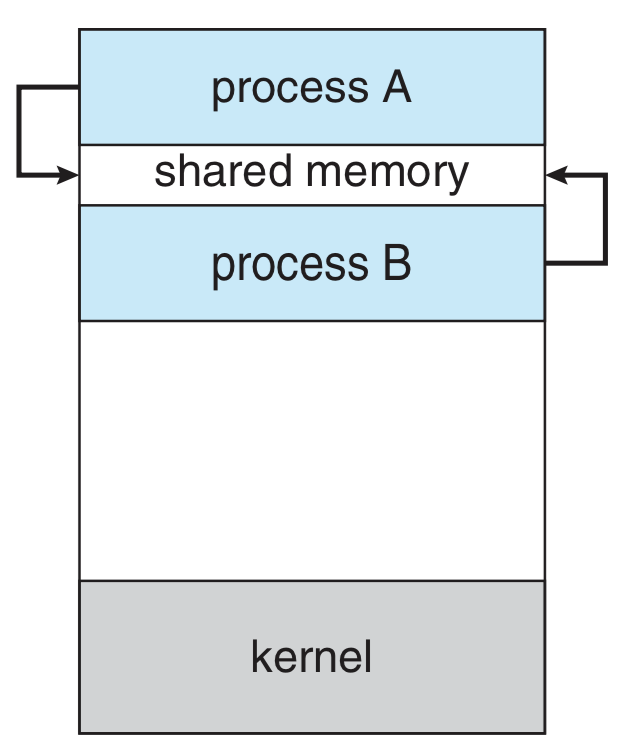
\includegraphics[width=0.2\textwidth]{images/shared-memory.png}\\
	A view of memory when a block is designated as shared~\cite{osc}.
\end{center}

Note that in the diagram the shared memory area appears in between the memory for processes $A$ and $B$; this is not necessarily the case (the shared block could be anywhere). It tends to be in the block for the process that creates the shared memory in the first place. This makes sense, because Process $A$ will request the memory from the operating system and then ask the OS to consider a particular block $A$ already owns to be shared.

When a section of memory is shared, there exists the possibility that one process will overwrite another's changes. To prevent this sort of problem, we will need a mechanism for co-ordination... a subject we will return to later.

\subsubsection*{File System}

Another way for two processes to communicate is through the file system. Unlike shared memory, messages stored in the file system will be persistent and survive a reboot. It can also be used when the sender and receiver know nothing about one another (and the programmer knows nothing about proper IPC mechanisms).

Rather than asking the operating system to get involved with shared memory and being concerned about which programs have access to it, the producer may write to a file in an agreed upon location and the consumer may read from that same location. The operating system is still involved because of its role in file creation and manipulation (as well as permissions for who may read and write a file).

If one file is being used then we still have the problem of co-ordination: making sure one process does not overwrite the changes of another. We can get around this, however, by using multiple files with unique IDs. Consider an example from a co-op work term: if the producer is generating XML data, it can write in a file in a designated \texttt{import/} directory. The consumer program scans the directory, and when it finds files, reads the file and imports the data contained therein. The imported data is then shown in the program. In this case, since one process writes files and another reads them, there is no possibility that one process overwrites the data of another. As long as the sender chooses distinct file names, it will not overwrite a message if a second message is created before the receiver picks up the first.

\subsubsection*{Message Passing}

Message passing is a service provided by the operating system where the sender will give the message to the OS and ask that it be delivered to a recipient. There are two basic operations: sending and receiving. Messages can be of fixed or variable size.

Our experience with postal mail, or e-mail, suggests that to send a message successfully, the sender needs to indicate where the message should go. Under \textit{direct communication}, each process that wants to communicate needs to explicitly name the recipient or sender of the communication, making the send and receive functions~\cite{osc}:\\
\texttt{send(A, message)} -- Send a message to process $A$.\\
\texttt{receive(B, message)} -- Receive a message from process $B$.

This requires \textit{symmetric} addressing: the sender and receiver have to know one another to communicate. This deviates from our experience in sending postal mail: receiving an item does not require foreknowledge of the sender. We would more typically expect \textit{asymmetric} addressing: the sender names the recipient, but the receiver can pick up items from anyone. The system calls for that scheme are~\cite{osc}:\\
\texttt{send($A$, message)} -- Send a message to Process $A$ (unchanged).\\
\texttt{receive(id, message)} -- Receive a message from any process; the variable \texttt{id} is set to the sender.

In either case, we have to know some identifier for the other processes. This is not very flexible; if we want to replace process $B$ with some alternative software, do we have to change the identifier in $A$, recompile it, and reinstall it? Do we ``fake'' the identifier of the new software so it calls itself $B$ even though it's not the same software? Furthermore, oftentimes  the sender will produce the data but is not interested in who receives it. 

What we would like is \textit{indirect communication} where the messages are sent to mailboxes. That makes our send and receive functions~\cite{osc}:\\
\texttt{send(M, message)} -- Send a message to mailbox $M$.\\
\texttt{receive(M, message)} -- Receive a message from mailbox $M$.

A mailbox may belong specifically to one process or may be set up by the operating system. If the mailbox belongs to the process, then anyone can send to this mailbox, but only the owning process may receive messages from that mailbox. If the owner process has not started or has terminated, attempting to send to that mailbox will be an error for the sender.

If the mailbox is owned by the operating system, it is persistent and independent of any particular process. When we used direct communication, e.g., sending to process $A$, the communication relationship is 1:1 - one sender and one receiver. When there was a mailbox owned by $A$, we could be certain that only process $A$ could retrieve items from that mailbox. There is no conceptual reason, however, preventing an operating system mailbox from belonging to more than one process. If mailbox $M$ belongs to the operating system and processes $P_{1}$ and $P_{2}$ have access to it, which process will receive a message sent to that mailbox?

There are two ways we can deal with this problem. The first is that the OS should allow only one process at a time to pick up items from the mailbox, thus preventing the problem altogether. The other solution is that the OS may have some scheme: whichever process gets there first, alternation (taking turns), or any other system of deciding whose turn it is.

The diagram below shows a message queue for communication between processes $A$ and $B$:
\begin{center}
	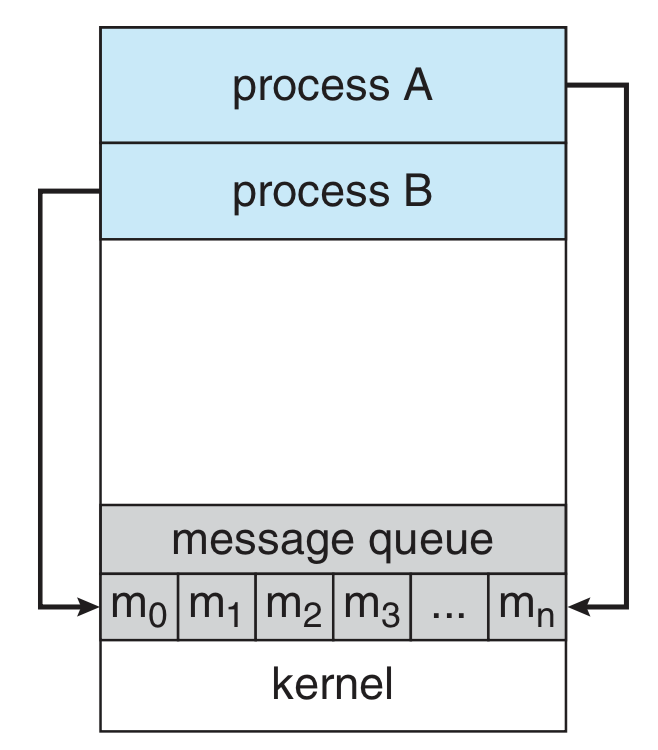
\includegraphics[width=0.2\textwidth]{images/message-passing.png}\\
	A view of memory in a message-passing system~\cite{osc}.
\end{center}

In this diagram we see something new for the receiver process: a message queue.

\subsection*{Message Queues}

Thus far we have dealt with messages one at a time: the sender wants to send one message and the receiver wants to receive one message. If the sender wants to send a second message before the first message is received, the sender will have three choices, regardless of whether the communication is synchronous:

\begin{enumerate}
	\item Wait for the last message to be picked up (block).
	\item Overwrite the last message (sometimes this is what you want).
	\item Discard the current message (let the old one remain).
\end{enumerate}

A message queue may alleviate the problem or just ``kick the can down the road''. If a queue exists, when sending a message, that message is placed in the queue and when receiving a message, the first message is taken. If the queue is of (effectively) unlimited size, then the problem may generally be ignored. If the queue has a fixed size then the problem is put off but not solved: the sender can keep adding messages to the queue until the queue is full. If the queue is full, the sender has to face the same choices of what to do: block, overwrite, or discard.

\subsubsection*{UNIX Pipes}

In UNIX, we can create a \textit{pipe} to set up communication between a producer and consumer. The producer writes in one end of the pipe and the consumer receives it on the other. This is unidirectional, so if bidirectional communication is desired, two pipes must be used (going in different directions). The UNIX method for creating a pipe is \texttt{pipe} and it is constructed with the call \texttt{pipe( int fileDescriptors[])} where \texttt{fileDescriptors[0]} is the read-end and \texttt{fileDescriptors[1]} is the write-end~\cite{osc}. Yes, \texttt{fileDescriptors} means that UNIX thinks of a pipe as a file (UNIX thinks \underline{everything} is a file...) even though it is in memory.

\begin{center}
	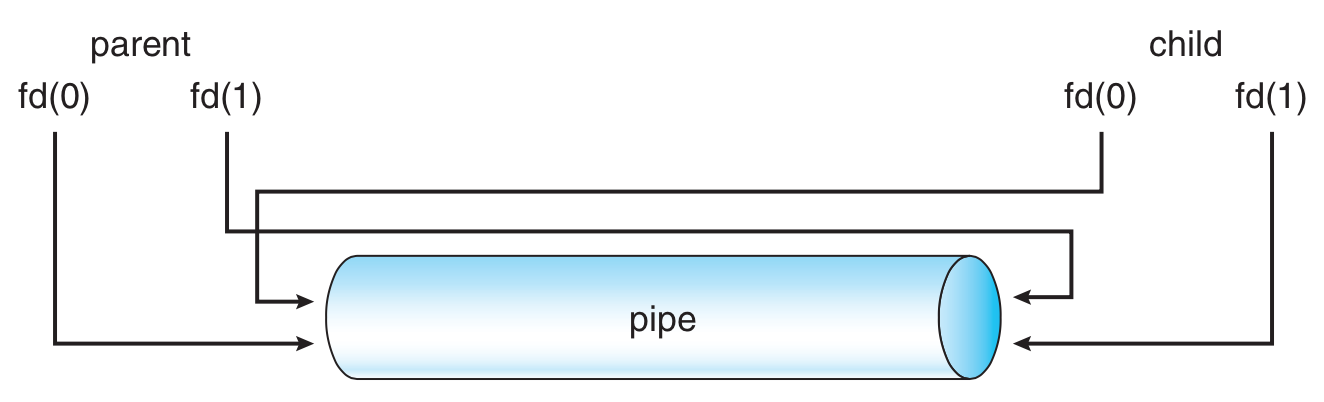
\includegraphics[width=0.5\textwidth]{images/unix-pipe.png}\\
	A UNIX Pipe~\cite{osc}.
\end{center}

The pipe itself is a block of main memory that is interpreted as a circular queue, and each entry in the queue is fixed in size and usually one character. The sender may place the message into the queue in small chunks, but the receiver gets data one character at a time. Thus, the sender and receiver need to know when the message is finished. This may be through the use of a designated termination character (e.g., the line feed or null character), or the message may begin with an explicit value of the number of characters the message will be~\cite{mte241}.

A UNIX pipe may be stored on disk. When this happens, we call it a \textit{named pipe}. Unless we make it a named pipe, a pipe exists only as long as the processes are communicating. Furthermore, regular pipes depend on file descriptors, so a parent-child relationship is required to get the descriptors from one process to another. The named pipe, however, might be used by any process and will persist even after the creating process has terminated. Another nice bonus of named pipes is that they can be bidirectional, so we do not need two pipes for communication to go in both directions. With that said, communication can only go in one direction at a time; if concurrent communication is required, a second pipe is needed after all.

You may have worked with pipes on the UNIX command line. A command like \texttt{ cat fork.c | less } creates a pipe that takes the output of the \texttt{cat} program and delivers it as input to the program \texttt{less} which allows for scrolling and pagination of that data.

\subsubsection*{UNIX Pipes: Code Example}

Let's consider an example from~\cite{osc} that combines the pipe concept with what we've seen before: using \texttt{fork} to spawn a new child process and then setting up a communication pipe between the parent and child. We will send a message ``Greetings'' from the parent to the child.

\begin{verbatim}
#include <sys/types.h> 
#include <stdio.h> 
#include <string.h> 
#include <unistd.h>

#define BUFFER_SIZE 25
#define READ_END 0 
#define WRITE_END 1

int main(void)
{
  char write_msg[BUFFER_SIZE] = "Greetings"; 
  char read_msg[BUFFER_SIZE];
  int fd[2];
  pid_t pid;

  if (pipe(fd) == -1) {
    fprintf(stderr,"Pipe failed");
    return 1;
  }
  
  /* fork a child process */
  pid = fork();
  
  if (pid < 0) { 
    /* error occurred */ 
    fprintf(stderr, "Fork Failed"); 
    return 1;
  }

  if (pid > 0) { /* parent process */
    /* close the unused end of the pipe */ 
    close(fd[READ_END]);
    
    /* write to the pipe */
    write(fd[WRITE_END], write_msg, strlen(write_msg)+1);
    
    /* close the write end of the pipe */
    close(fd[WRITE_END]);
    
  } else { /* child process */
    /* close the unused end of the pipe */ 
    close(fd[WRITE_END]);
    
    /* read from the pipe */
    read(fd[READ_END], read_msg, BUFFER_SIZE); 
    printf("read %s",read_msg);
     /* close the write end of the pipe */
     close(fd[READ_END]);
  }
  return 0;
}
\end{verbatim}

If we wanted to create a named pipe, the system call for that is \texttt{mkfifo} (make first-in-first-out) because sometimes a named pipe is called a FIFO. As it is a file, it can be manipulated with the usual UNIX file system calls: \texttt{open}, \texttt{read}, \texttt{write}, and \texttt{close}~\cite{osc}.

\bibliographystyle{alphaurl}
\bibliography{252}


\end{document}